\begin{slide}{X-ray Absorption Fine-Structure Spectroscopy}
    
  X-ray Absorption Fine-Structure ({\Blue{XAFS}}) is the modulation of
  the x-ray absorption coefficient $\mu(E)$ at energies near and above a
  core-level electron binding energy.

\begin{tabular}{ll}
  \begin{minipage}{52mm}
    \begin{center}
      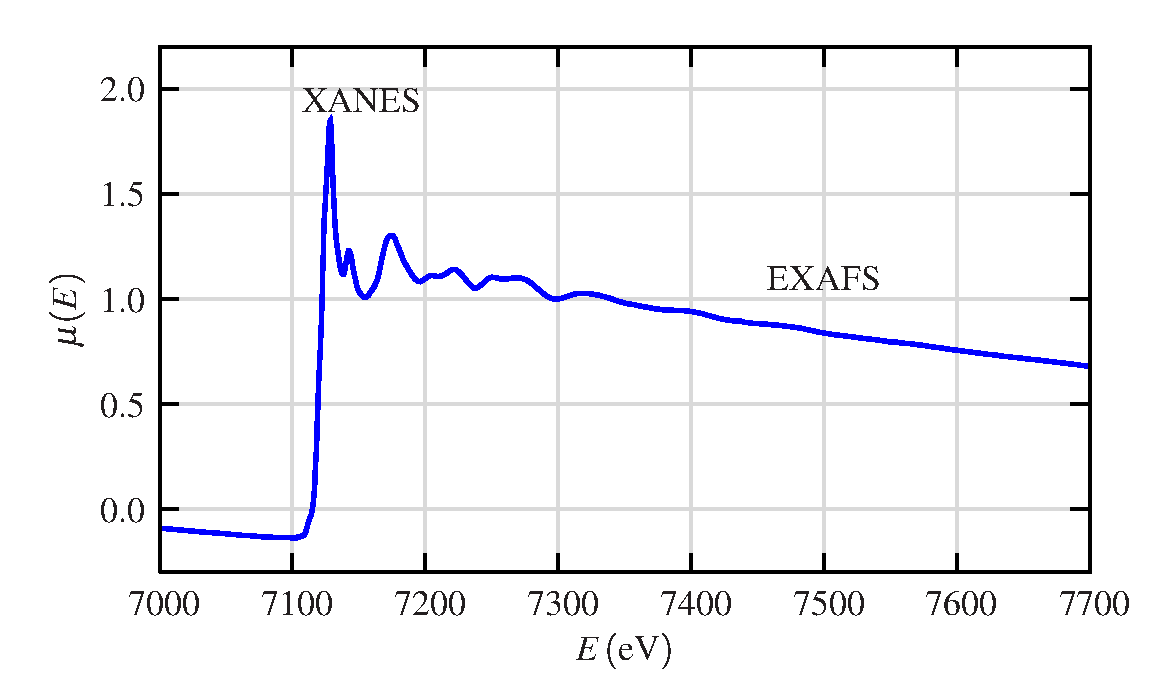
\includegraphics[width=53mm]{figs/general/feo_mu}
    \end{center}
    {\tiny{
        \hspace{5mm} {\Red{XANES}} = {\Red{X}}-ray {\Red{A}}bsorption {\Red{N}}ear-{\Red{E}}dge {\Red{S}}pectroscopy
        
        \hspace{5mm} {\Red{EXAFS}} = {\Red{E}}xtended {\Red{X}}-ray {\Red{A}}bsorption   {\Red{F}}ine-{\Red{S}}tructure
      }}
    \vspace{9mm}
  \end{minipage} 
  & 
  \begin{minipage}{53mm}
    {\tiny{
        \begin{entry}
      \pause
    \item[{\Red{Any Element}}]  $Z \gtrsim 4$, depending on source.
      \pause
    \item[{\Red{Element Specific}}]  element of interest is selected
      from core-level energy.
      \pause  
    \item[{\Red{Valence Probe}}] XANES gives chemical state and
      formal valence.
      \pause
    \item[{\Red{Local Structure Probe}}] EXAFS gives atomic species,
      distance, and coordination number of neighbor atoms within 5 {\AA}
      of absorbing atom.
      \pause
    \item[{\Red{Low Concentrations}}] down to $\sim$1ppm.
      \pause
    \item[{\Red{Minimal Sample Needs}}] crystallinity is not required: 
      liquids, solutions, glasses, soils, surfaces, \ldots.
      
    \end{entry}
  } }
\end{minipage} \\
\end{tabular}

\vmm\pause

XAFS can be combined with other conditions: {\emph{in-situ}}, with
micron-sized x-ray beams, at extreme conditions (temperature,
pressure), or with time resolution.      


\vfill
\end{slide} 
